\documentclass[a4paper,11pt]{article}

\usepackage[margin=3cm]{geometry}

\usepackage{graphicx}
\usepackage{subcaption}
\usepackage[colorlinks,allcolors=violet]{hyperref}
\usepackage{url}
\usepackage{lmodern}
\usepackage[dutch]{babel}

% https://tex.stackexchange.com/questions/94032/fancy-tables-in-latex
\usepackage[table]{xcolor}
\usepackage{booktabs}

\usepackage[utf8]{inputenc}

% https://tex.stackexchange.com/questions/664/why-should-i-use-usepackaget1fontenc
\usepackage[T1]{fontenc}
\usepackage{microtype} % good font tricks

\newcommand{\note}[1]{{\colorbox{yellow!40!white}{#1}}}
\newcommand{\exampletext}[1]{{\color{blue!60!black}#1}}

\begin{document}

\noindent
\colorbox[HTML]{52BDEC}{\bfseries\parbox{\textwidth}{\centering\large
  --- Verslag P\&O CW 2019--2020 Taak 5 ---
}}
\\[-1mm]
\colorbox[HTML]{00407A}{\bfseries\color{white}\parbox{\textwidth}{
  Department Computerwetenschappen -- KU Leuven
  \hfill
  \today
}}
\\

\smallskip

\noindent

\begin{tabular}{*4l}
\toprule
\multicolumn{2}{l}{\large\textbf{Team 12}} \\
\midrule
Frédéric Blondeel & h \\
Martijn Debeuf & h \\
Toon Sauvillers & h \\ % fill in the time spend on this task per team member who worked on it
Dirk Vanbeveren & h \\
Bert Van den Bosch & h \\
Seppe Van Steenbergen & h \\


\bottomrule
\hline
\end{tabular}\\

\noindent
{\color[HTML]{52BDEC} \rule{\linewidth}{1mm} }
\tableofcontents
\newpage
\section{Introductie}\label{sec:introductie}
Nu de schermen gevonden en geidentificeerd zijn kan men wat meer dan lijntjes displayen. Met deze taak zullen verschillende schermen gebruikt worden om een grotere foto te tonen. Het is dus mogelijk om enkele gsm's samen één image te tonen, verspreid over de displays. Hiervoor world gebruik gemaakt van perspectief veranderende matrices, server/client communicatie, etc.

% !TeX spellcheck = de_DE
\section{Delaunay triangulatie}
Om verschillende punten mooi te verbinden, kan er gebruik gemaakt worden van een Delaunay triangulatie. Deze wordt toegepast op de middelpunten van de schermen. Wanneer deze triangulatie geprojecteerd wordt, zullen de liggingen van de schermen mooi worden weergegeven. Bij een Delaunay triangulatie worden alle punten zo verbonden dat ze verscheidene driehoeken vormen. De zijden mogen niet overlappen en de kleinste hoek in de configuratie moet maximaal zijn. \cite{delaunaywiki}

De triangulatie kan op vele manieren worden berekend, in dit verslag zijn er twee soorten algoritmen onderzocht. Het S-hull algoritme en het Boyler-Watson algoritme.

\subsection{S-hull}
Het eerste algoritme is het S-hull algoritme. Het is een $O(nlog(n))$ algoritme, gebruikmakend van een radiaal propagerende sweep hull. S-hull start met twee punten, één daarvan is willekeurig geselecteerd. Het tweede punt is het dichtsbijzijnde. Vervolgens zal er een derde worden gezocht dat samen met de twee voorgaande een zo klein mogelijke cirkel maakt. Het middelpunt van deze cirkel wordt gebruikt om alle punten te sorteren t.o.v. de afstand met het gevonden middenpunt. Deze gesorteerde punten zullen één voor één toegevoegd worden aan de configuratie.

Nadat ze sequentieel zijn toegevoegd, is er een niet overlappende triangulatie bekomen. Om een Delaunay triangulatie te bekomen moet er echter ook gekeken worden naar de hoeken. Elke driehoek zal nu worden afgegaan en er wordt gekeken of er geen andere driehoek kan gevormd worden met de buurdriehoeken zodat de minimale hoek gemaximaliseerd wordt, zie figuur \ref{driehoekswitch}. \cite{s-hull}
\begin{figure}

	\center
	\begin{subfigure}{0.4\textwidth}
		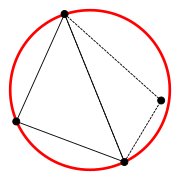
\includegraphics[width=\textwidth]{slechte_driehoek}
		\caption{De twee buurdriehoeken blijken niet ideaal te zijn.}
	\end{subfigure}
	\begin{subfigure}{0.4\textwidth}
		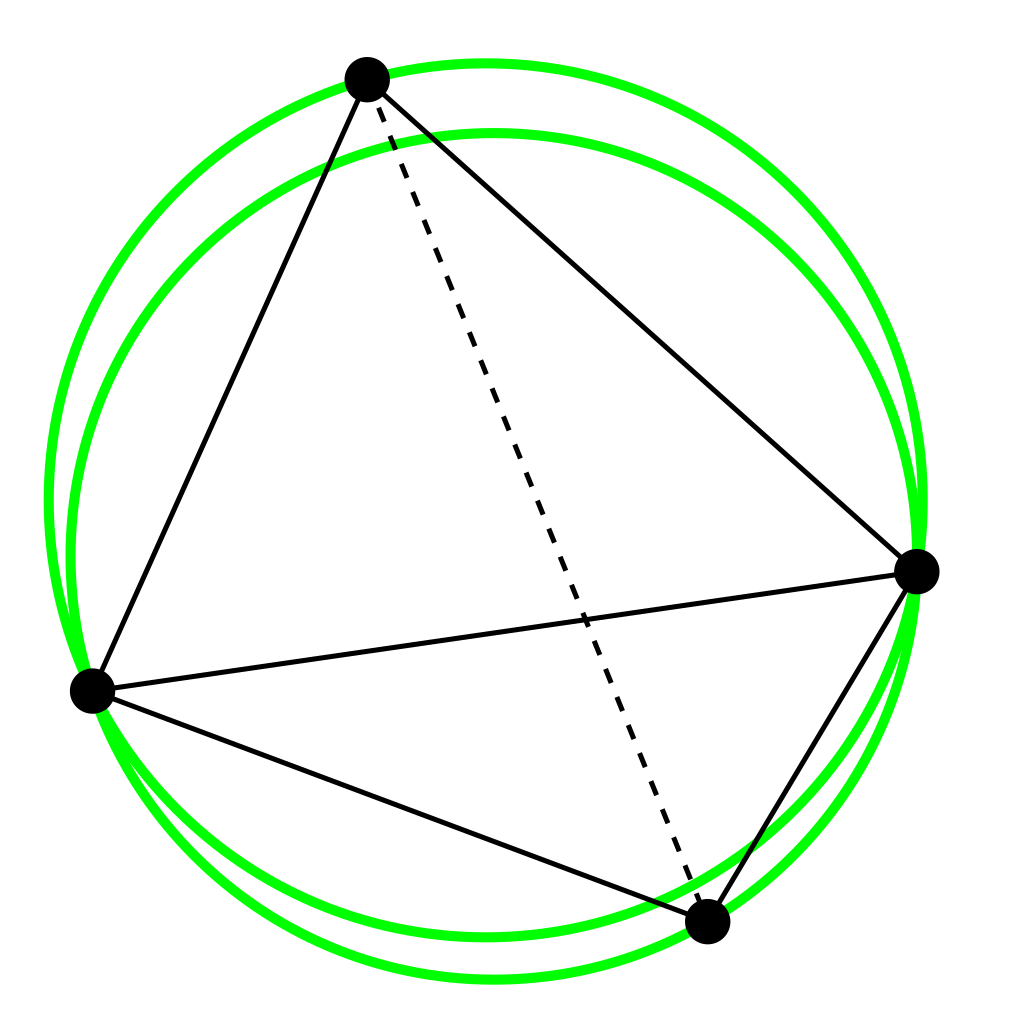
\includegraphics[width=\textwidth]{goede_driehoek}
		\caption{De twee buurdriehoeken maximaliseren met een andere verbinding de kleinste hoek.}
	\end{subfigure}
	\caption{Het maximaliseren van de kleinste hoek \cite{delaunaywiki}}
	\label{driehoekswitch}
\end{figure}

Dit algoritme is echter niet gebruikt. Ook al is het algoritme $O(nlog(n))$ het vereist een zeer goede data management om deze snelheid te behalen.  \cite{Lund2014} Er is daarom gekozen voor een simpeler algoritme, namelijk het Boyler-Watson algoritme.

\subsection{Bowyer-Watson}
Het Bowyer-Watson algoritme is wel geïmplementeerd. Het heeft een tijdscomplexiteit van $O(n^2)$, dit is aanzienlijk trager dan het S-hull algoritme. \cite{Bowyer-WatsonWiki} Het vereist echter een minder complex data management en is daarom ook makkelijker te implementeren. De tijdscomplexiteit is ook relatief te zien, er zijn namelijk maar maximaal 120 detecteerbare schermen. Meer kunnen er door het identificatiemechanisme niet worden gevonden. Gezien het laag aantal punten, moet het algoritme niet nodeloos complex worden en kan er gekeken worden naar `tragere' methoden, zoals deze Bowyer-Watson.

\paragraph{}
Bowyer-Watson gaat er van uit dat punten enkel worden toegevoegd in een al bestaande Delaunay triangulatie. Als eerste worden er twee superdriehoeken gezocht. Deze driehoeken zullen alle te trianguleren punten bevatten. De implementaties waarop het algoritme is gebaseerd \cite{Bowyer-WatsonWiki} \cite{bowyer-watsonImplementation} stelden beiden een `superdriehoek' voor, zie figuur \ref{bowyer-watson-a} Echter is het eenvoudiger om een omkaderende vierhoek te vormen en deze op te delen in twee driehoeken. Vervolgens worden alle punten één voor één toegevoegd.

Voor elk punt worden alle driehoeken gezocht waarvan het punt in de omschreven cirkel zit. Wanneer twee driehoeken eenzelfde zijde delen, wordt deze verwijderd. Alle punten van de omschreven veelhoek van de twee driehoeken worden nu verbonden met het toegevoegde punt, zie figuur \ref{bowyer-watson-b}. Met deze werkwijze zal er op elk moment een Delaunay triangulatie zijn en moeten de driehoeken achteraf niet meer overlopen worden. Met het gevolg dat het data management voor deze methode minder complex is.

Eens alle punten toegevoegd zijn, worden de driehoeken die één of meer hoeken van de omkaderende vierhoek bevatten verwijderd, zie figuur \ref{bowyer-watson-c}. Aangezien deze driehoeken aan de buitenkant liggen is dit toegestaan. Er zal een Delaunay triangulatie overblijven van alle onderzochte punten.

\begin{figure}
	\center
	\begin{subfigure}{0.4\textwidth}
		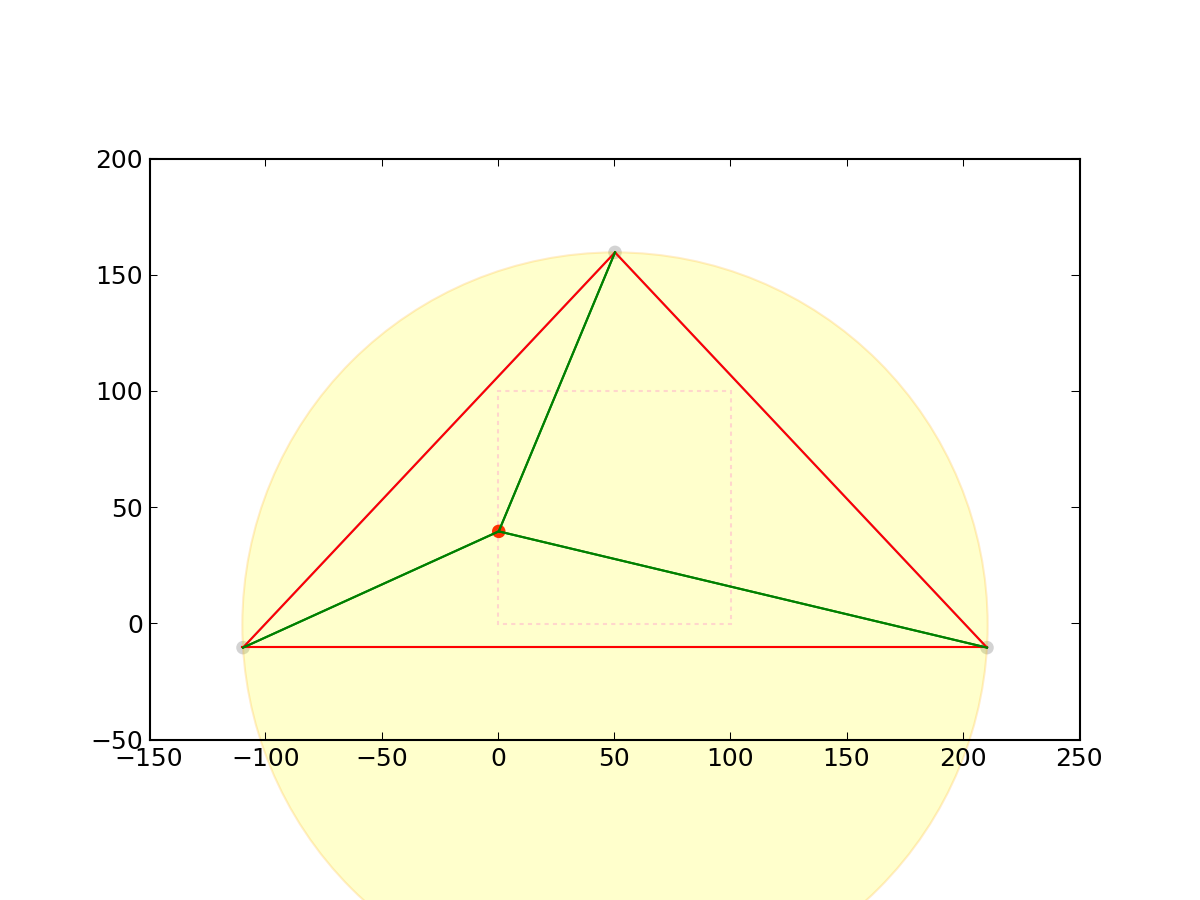
\includegraphics[width=\textwidth]{bowyer-watson_superdriehoek}
		\caption{De rode superdriehoek waarin alle punten zullen worden toegevoegd.}
		\label{bowyer-watson-a}
	\end{subfigure}
	\begin{subfigure}{0.4\textwidth}
		\includegraphics[width=\textwidth]{bowyer-watson_nieuwpunt}
		\caption{Een nieuw punt wordt toegevoegd. In geel de omschreven cirkels. De gestippelde zijde wordt verwijderd, de groene toegevoegd.}
		\label{bowyer-watson-b}
	\end{subfigure}
		\begin{subfigure}{0.4\textwidth}
		\includegraphics[width=\textwidth]{bowyer-watson_verwijderen}
		\caption{In rood alle driehoeken verbonden met de superdriehoek, deze worden uiteindelijk verwijderd.}
		\label{bowyer-watson-c}
	\end{subfigure}
	\caption{Het Bowyer-Watson algoritme \cite{Bowyer-WatsonWiki}}
	\label{bowyer-watson}
\end{figure}

\subsection{Algemeen concept}
De testen maken gebruik van een simpele server waar clients op kunnen verbinden. De client kan vervolgens het absolute tijdverschil meten met een atomische wereldklok.

Eerst en vooral is er een vertraging tussen een aangesloten client en de server, de {\it ping}. Dit is gemeten in milliseconden. De testen meten de vertraging door een bericht met de actuele tijd te verzenden van de server naar de client, en terug. De vertraging is dan de verzonden tijd afgetrokken van de actuele tijd waarmee de ping verkregen is.
In figuur \ref{ping} is de informatieoverdracht zichtbaar. De server berekent de servertijd (TS1) door middel van een API die de exacte wereldtijd teruggeeft, verzonden naar de client en teruggekregen. De uiteindelijke ping is: \[ping = TS2 - TS1\] met TS2 de actuele tijd berekent in de server TS2

\begin{figure}[h]
\centering
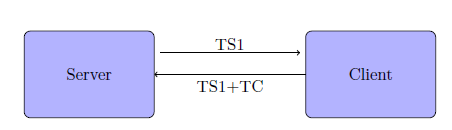
\includegraphics[scale=0.8]{img/img.png}
\caption{Ping} \label{ping}
\end{figure}


Het is niet gegarandeerd dat de klokken van de clients allemaal gesynchroniseerd zijn met de server. Bij het terug verzenden van de client naar de server wordt de clienttijd (TC) bij het bericht gezet.  Met deze TC en de berekende {\it ping} is het mogelijk het tijdsverschil tussen de client en de server te bepalen ($DeltaTime$).
\[DeltaTime = (TC+ping/2) - TS2\]
Deze data wordt vervolgens tussen verschillende browsers en besturingssystemen vergeleken.

\subsection{UDP vs TCP}

UDP heeft in tegenstelling tot TCP geen gevestigde verbinding nodig tussen bijvoorbeeld server en client. TCP zal garanderen dat data correct aankomt door middel van foutopsporing en zal ook in de goede volgorde binnenstromen. Om geen pakketten te verliezen zal TCP deze in een {\it receive buffer} steken en zal de applicatie de ontvangen data pas lezen als ze er klaar voor is. Tegenover UDP waar de data continu zal binnenstromen, ontvangen of niet. Deze zal ook niet aan foutopsporing doen en de juiste volgorde niet gegaranderen. Het is duidelijk dat UDP veel sneller is doordat deze minder stappen en controle bevat. Dit is ook de reden dat het NTP protocol UDP zal gebruiken in plaats van TCP. Het is logisch dat voor een simpele synchronisatie tussen client en server geen complex protocol nodig is. Socket.io gebruikt het TCP protocol in de browser voor veiligheidsredenen.

\subsection{Drift en skew}

Drift zal ervoor zorgen dat een klok niet meer synchroon met zijn oorspronkelijke referentie loopt. Windows lost dit op met een wekelijkse resync (het tijdsverschil zal dus op een sawtooth diagram lijken) terwijl Mac OSX rekening zal houden met de klok skew en andere hardware invloeden om zo beter synchroon te blijven.
Klok skew is het verschil van tijd van een kloksignaal tussen 2 componenten binnen een systeem(zie figuur \ref{skew1} \cite{skew}).

Het tijdsverschil van een windows computer en een atoomklok is gedurende 25 minuten gemeten (zie figuur \ref{drift}). De trendlijn is door de grafiek getrokken en het is duidelijk dat er geen effect ervan te zien is. Over langere tijdsperiode zal de drift groter worden, maar voor de animatie zal dit verwaarloosbaar zijn aangezien het onwaarschijnlijk is dat iemand dagenlang deze zal laten afspelen.

\begin{figure}[H]
\centering
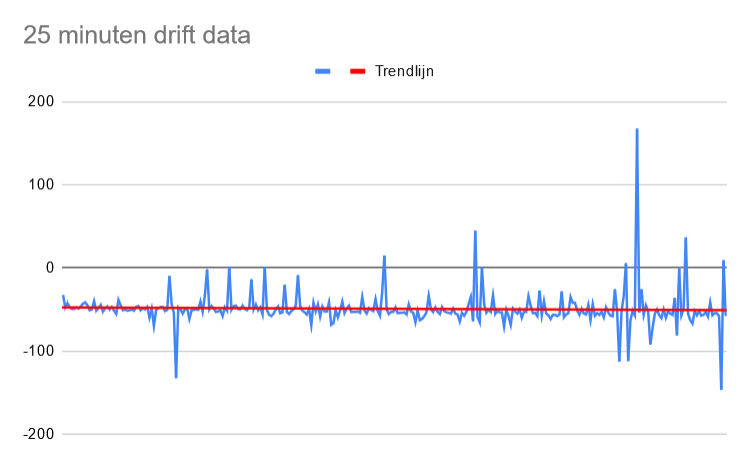
\includegraphics[scale=0.3]{img/drift.png}
\caption{Drift} \label{drift}
\end{figure}

\begin{figure}[H]
\centering
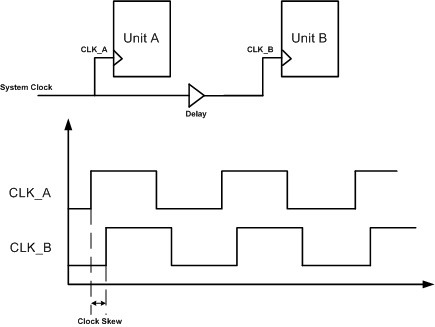
\includegraphics[scale=0.7]{img/skew.jpg}
\caption{Skew} \label{skew1}
\end{figure}


Klok skew kan problemen geven voor correct timings, en zoals eerder vermeld zal OSX dit tegen gaan via software. We zullen niet dieper gaan over de problemen van skew en OSX. 


\subsection{Analyse van de data}
\label{analyse}
Het is duidelijk dat er op elk soort systeem een afwijking gemeten wordt tegenover de referentieklok. Bij sommige operating systems al een groter verschil dan de andere, maar de reden waarom is niet altijd te verklaren of vrijgegeven en zullen hier dus niet verder op in gaan. Elk systeem wordt door het operating system zelf voldoende gesynchroniseerd met een server-klok als referentie en zou in principe maar een paar miliseconden mogen afwijken van deze referentieklok. De fout wordt pas waargenomen in de metingen van het verschil tussen de twee klokken over een netwerk. In deze situatie wordt er een poging gedaan om het verschil tussen device-klok en server-klok te vergelijken door de ping mee in rekening te brengen. De drift van beide klokken gaan over deze tijdsspanne minimaal zijn en gaan geen invloed hebben op deze verschillen. Bij de testen werd ook de gemiddelde ping en standaarduitwijking van de ping per test opgeslagen. Uit deze waarden valt af te leiden dat er bij grote pingfluctuaties ook een grote standaarduitwijking mee gepaard ging en wijst naar inconsistenties binnen het netwerk van ofwel de client ofwel de belasting op de server en is er bijgevolg meer kans op een grotere fout binnen de vergelijking van de klokken. 

\begin{figure}[H]
	\centering
	\begin{subfigure}{.5\textwidth}
		\centering
		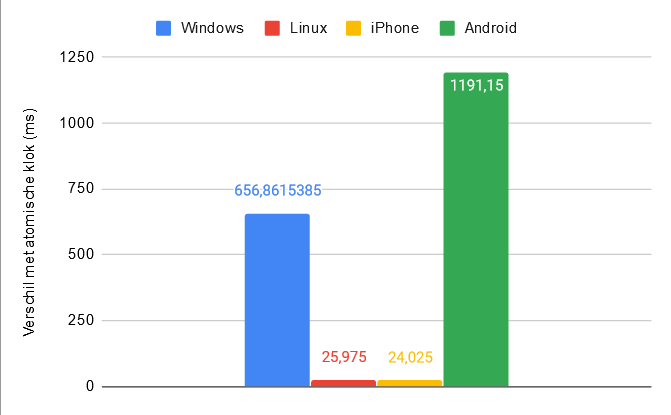
\includegraphics[width=.95\linewidth]{img/mediaan.png}
		\caption{Mediaan van tijdsverschil van elk device.}
		\label{fig:mediaan}
	\end{subfigure}%
	\begin{subfigure}{.5\textwidth}
		\centering
		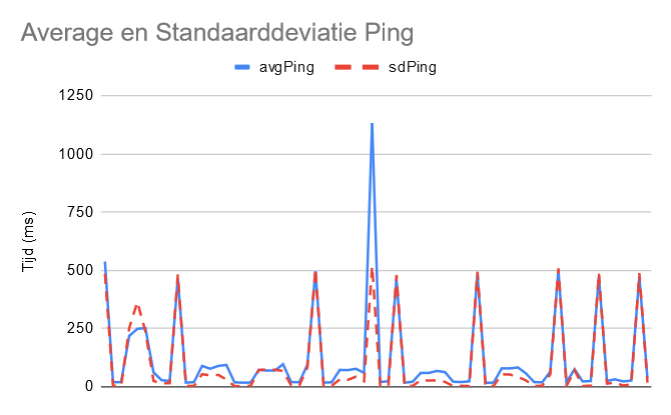
\includegraphics[width=.95\linewidth]{img/ping_results.png}
		\caption{Gemiddelde en standaarduitwijking van de ping met de server. }
		\label{fig:avgPing}
	\end{subfigure}
	\caption{Resultaten van de testen}
	\label{fig:results}
\end{figure}

In figuur \ref{fig:avgPing} is het duidelijk zichtbaar dat er een pieken zijn met hoge standaardafwijkingen. Dit wilt zeggen dat er heel grote fluctuaties zijn in de ping tijdens het synchronisatie proces met 10 opmetingen. Hiermee is de gesynchroniseerde tijd een afwijking hebben met de werkelijke tijd tot ($maxPing - minPing$).





















\section{Valkuilen}
In theorie kan er van elke opstelling waarbij de punten niet allemaal colineair zijn een triangulatie worden gevonden, zie figuur \ref{colineair}. Echter door afronding bij de berekeningen zal er bij bijna colineaire punten geen juiste  configuratie gevonden worden, zie figuur \ref{almost_colineair}. 

\begin{figure}
	\center
	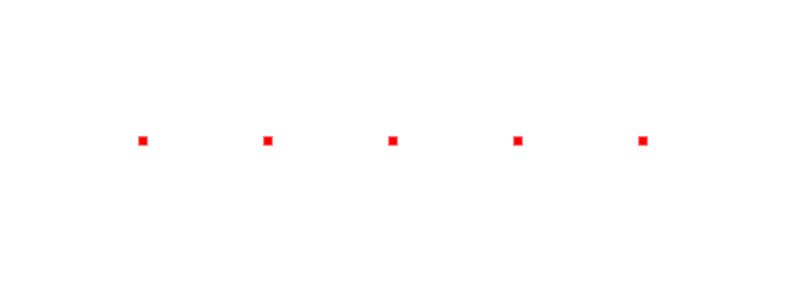
\includegraphics[width=0.4\textwidth]{colineair}
	\caption{Van colineaire punten kan geen triangulatie gevonden worden.}
	\label{colineair}
\end{figure}
\begin{figure}
	\center
	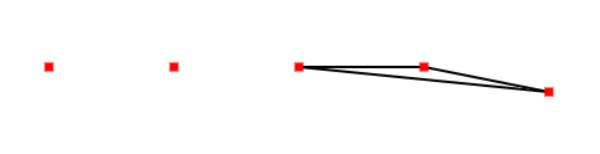
\includegraphics[width=0.4\textwidth]{almost_colinair}
	\caption{Van bijna colineaire punten kan geen triangulatie gevonden worden door afrondingsfouten bij berekeningen.}
	\label{almost_colineair}
\end{figure}

\section{Besluit}\label{sec:besluit}
 
Uit de bevindingen is gebleken dat de interpretatie van kleur sterk afhankelijk is van de manier waarop kleur wordt voorgesteld en de omgevingsfactoren die hierbij aanwezig zijn. Enerzijds speelt de kleurruimte waarin een kleur wordt voorgesteld een grote rol bij de detectie. Van de verschillende kleurruimten die bekeken zijn, is er niet een die eenduidig beter is dan de andere. Beiden hebben hun voordelen, zo is HSL beter voor de detectie van alle kleuren dan RGB. Maar de detectieratio van zwart en wit is dan wel weer aannoemelijk beter in RGB dan in HSL.  Anderzijds spelen omgevingsfactoren ook een belangrijke rol bij de detectie van de kleuren. Hiervoor werd gekeken naar zowel de omgeving, de lichtinval en de helderheid van het scherm. De belangrijkste bevindingen hierbij hebben te maken met de lichtinval en de omgeving. Door lichtinval komt er bij artificieel licht extra rood in de kleuren door de rode schijn die het licht achterlaat. Hoe groter de omgeving, hoe meer de kleuren fout gedetecteerd gaan worden. Dit is te wijten aan het feit dat de camera hierbij op de omgeving gaat focussen in plaats van op het scherm. Tot slot is ook gebleken dat helderheid geen groot effect heeft op de detectie.

\newpage

\bibliographystyle{unsrt}
\bibliography{bibliography}



\end{document}